\section{Introduction}
Nowadays, semantic segmentation applied to still 2D images, video, and even 3D or volumetirc data is one of the key problems in the field of computer vision.
Especially, video objects segmentation is one of the high-level task, which can greatly improve the human knowledge on video understanding.
Recently, increasing attention are paid in autonomous driving\cite{geiger2012we, cordts2016cityscapes, ess2009segmentation}, 
which is regarded as the most challenging part in visual understanding. 
Such problem has been addressed in the past using various traditional computer vision techniques, which cannot slove the problem clearly because of large amounts of video sequence data.
Deep learning has turned that table because of the extremely strong feature respresentation power. 
Far from now, it's proved that deep convolutional neural network \cite{farabet2013learning, ning2005toward} figure the video objects segmenation well in many applications and have excellent
performance in terms of accuracy and efficiency. 

In last few years, video object segmentation make an impressive progress due to the existence of excellent large scale video datesets \cite{DAVIS2016, SegTrack, Youtube}, which provide a densely
accurate labeling groundtruth. A lots of work mainly address problems on video instance segmentation and primary object segmentation in DAVIS challenges setting. So this survey mainly revise some 
excellent works on recent popular video objects segmentation topics.

To the best of our knowledge, this is the first review to focus on deep learning for video objects segmentation mainly based on DAVIS challenges setting. In contrast to this survey, there lots of 
semantic segmentation survey, which mainly apply the object segmentation on still 2D images. Howerver, video sequences have abundunt information in temporal diemension. Many techniques can utilize
the more motion cues besides apperances cues. So the most methods are introduced here that combine spatial-temporal information together, which will give greatly benefits to tackle video objects 
segmentation. 

In Fig.\ref{VOS}, we introduced three different setting(all based on DAVIS challenges setting): Semantic Semi-Supervised Video Object Segmenation(a.k.a Semantic Semi-Supervised setting) use object mask which in first frame to track the object in least frames; Instance Semi-Supervised Video Object Segmenation(a.k.a Instance Semi-Supervised setting) also use 
object mask which in first frame, which is same with Semantic Semi-Supervised setting, but there are multiple objects in first frame, and we need to differentiate each ohter; Unsupervised Video Obeject Segmentation(a.k.a Unsupervised setting) do not use any information about the tracked object, which just rely on motion and salient obejct as their prior knowledge.

\begin{figure*}[ht]
    \centering
    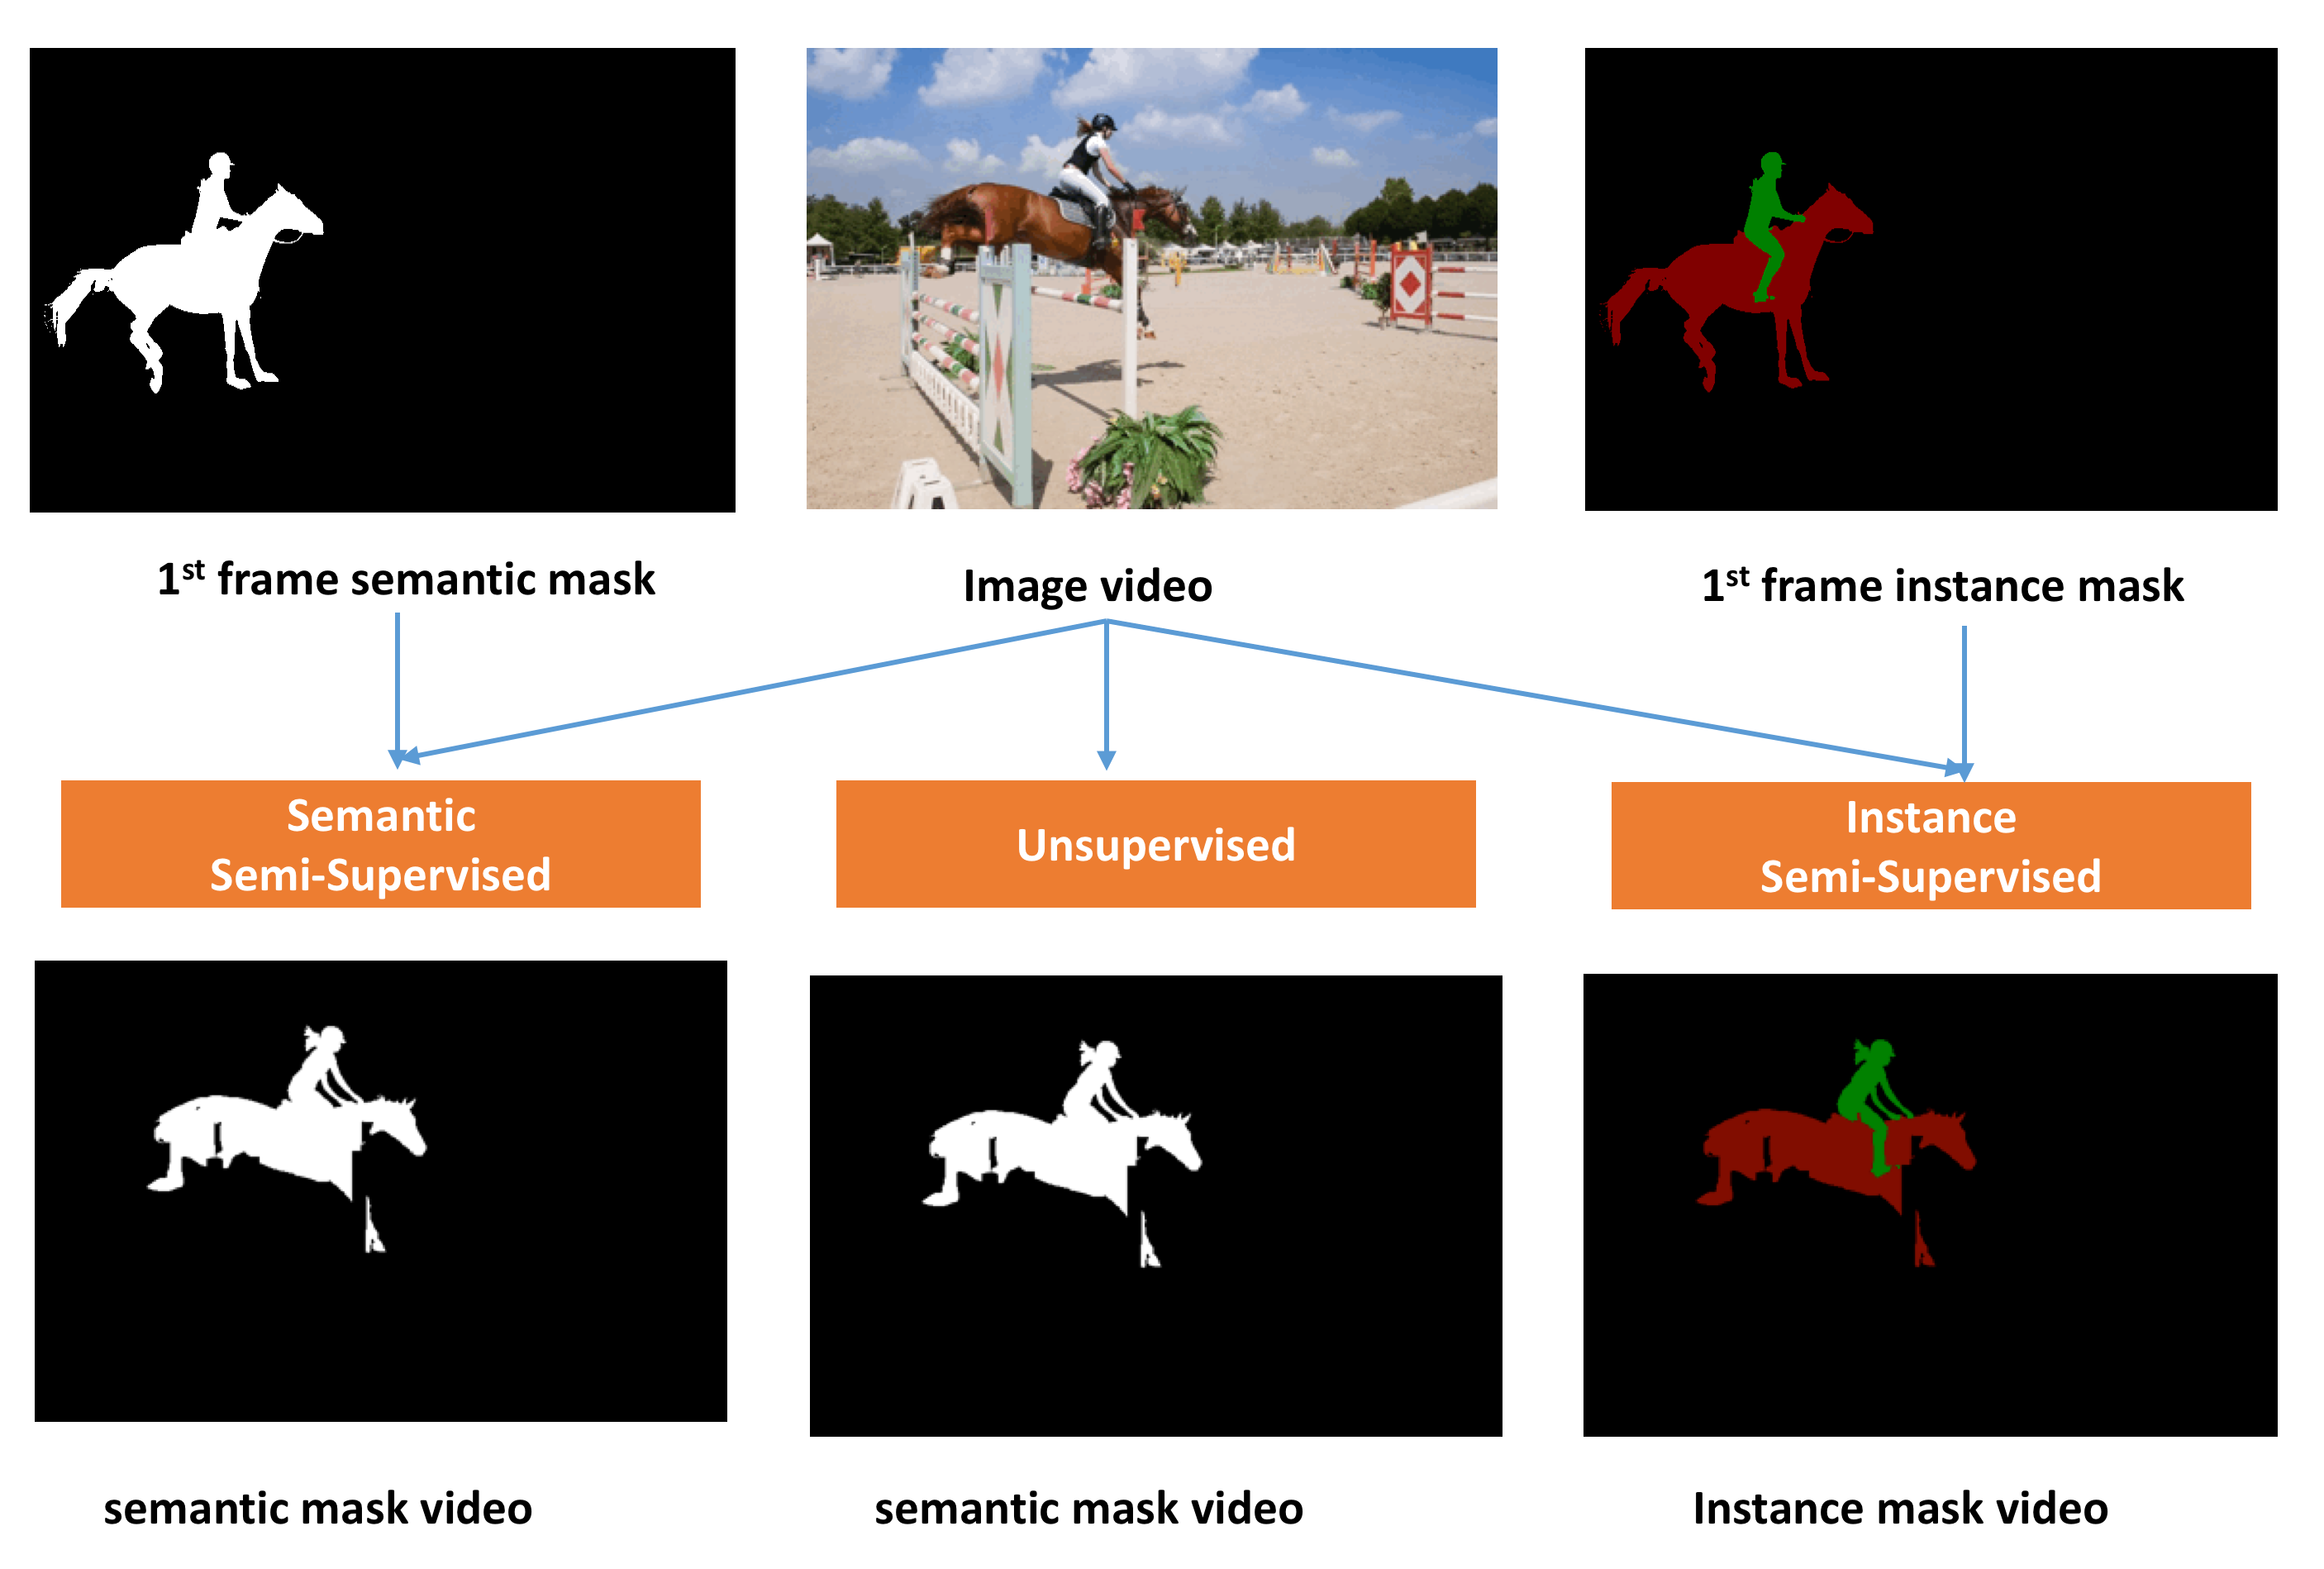
\includegraphics[width=\textwidth]{./figure/VOS.png}
    \caption{3 different setting in Video Object Segmentation: \textbf{Semantic Semi-Supervised Segmenation}(left), \textbf{Instance Semi-Supervised Segmentation}(right) and \textbf{Unsupervised Segmentation}(middle)}
    \label{VOS}
\end{figure*}


The key contributions of our work are as follows:
\begin{enumerate}
    \item  We provide a broad survey of existing network backbones and datasets that might be useful for video objects segmentation projects with deep learning techniques.
    \item  An in-depth and organized review of the most significant methods that use deep learning and combine spatial-temporal information for video objects segmentation, 
           their origins, and their contributions.
    \item  A thorough performance evaluation, which include the intersection of union and bounary accuracy.
    \item  A discussion about the aforementioned results, as well as a list of possible future works that might set the course of upcoming advances,
           and a conclusion summarizing the state of the art of the field.
\end{enumerate}


The remainder of this paper is organized as follows. Firstly, Section $2$ introduces the video objects segmentation problem as well as notation and conventions commonly used in the literature.
Other background concepts such as common deep neural networks and several specially techniques for videos are also reviewed. Next, Section 3 describes existing datasets and corresponding attributes.
section $4$ review some methods tackling video sequence based on different setting, semi-supervised and unsupervised ways. This section focus on descirbing the the contributions in papers and highlights some
specific techniques when dealing with videos sequences. Finally, Section 5 presents a brief discussion on the presented methods based on their quantitative results on the aforementioned datasets. 
In addition, future research directions are also laid out. At last, Section 6 summarizes the paper and draws conclusions about this work and the state of the art of the field.